\newpage
\section{Spesefikke anleggsvariasjonar}
\thispagestyle{fancy}

Sjølv om Sande reinseanlegg anvender \gls{SBR}-teknologi så er det enkle spesefikke
punkt der dette reinseanlegget avvik frå normalen. 
Sande reinseanlegg nyttar eksempelvis ein spesiell form for slambehandling sett i norsk perspektiv.

Vanleg slambehandling er deponering av slam som handterast og sendast til \gls{Hygienisering} \citep{Slam}. \newline
På Sande blir ikkje slammet lagra, men jamnlig spreid ut over eit bestemt område. På dette området er
det planta siv som skal ta opp slammet og resterande vatn blir naturleg filtrert og drenert.
Desse områda kallast sivbed.

Sivbeda er konstruert med fleire dreneringslag som gjer at resterande vatn skiljast ut i forskjellige soner.
Her kan desse handterast vidare etter ønska behov. 
Grunna denne slambehandlingsmetoden er det på Sande reinseanlegg heller slamfjerning frå reaktor
i reaksjonssekvens. Dette blir gjort for å ha mindre konsentrert slam \citep{MDPI}.

Sande reinseanlegg har fire sivbed og den kombinerte størrelsen er 676 $m^2$. Sivbeda er lokalisert på utsida av reinseanlegget (sjå figur~\ref{fig:Sivbed}).\newline
Videre har kvart sivbed sin eigen respektive ventil (sjå figur~\ref{fig:SivbedVentilar}), og under uttapping av slam vil kun eit sivbed og ein ventil vere aktiv. 
 

\begin{figure}[htbp]
    \centering
    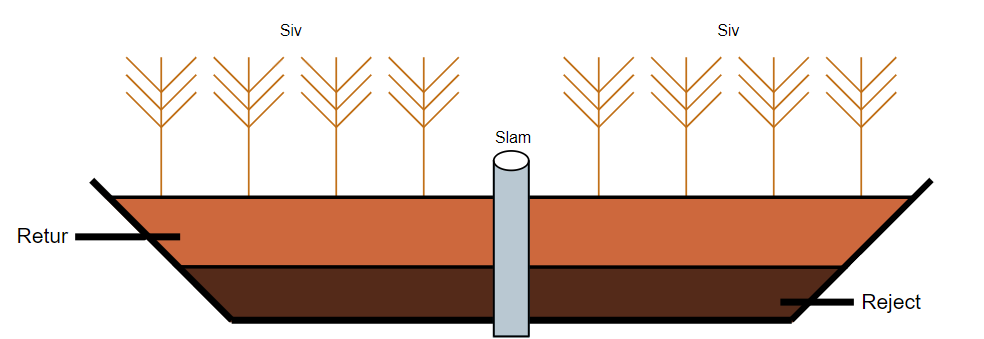
\includegraphics[width=1\textwidth]{Figurar/Sivbed.png}
    \caption{Illustrasjon sivbed}\label{fig:Sivbed}
\end{figure}

\newpage

\begin{figure}[htbp]
    \centering
    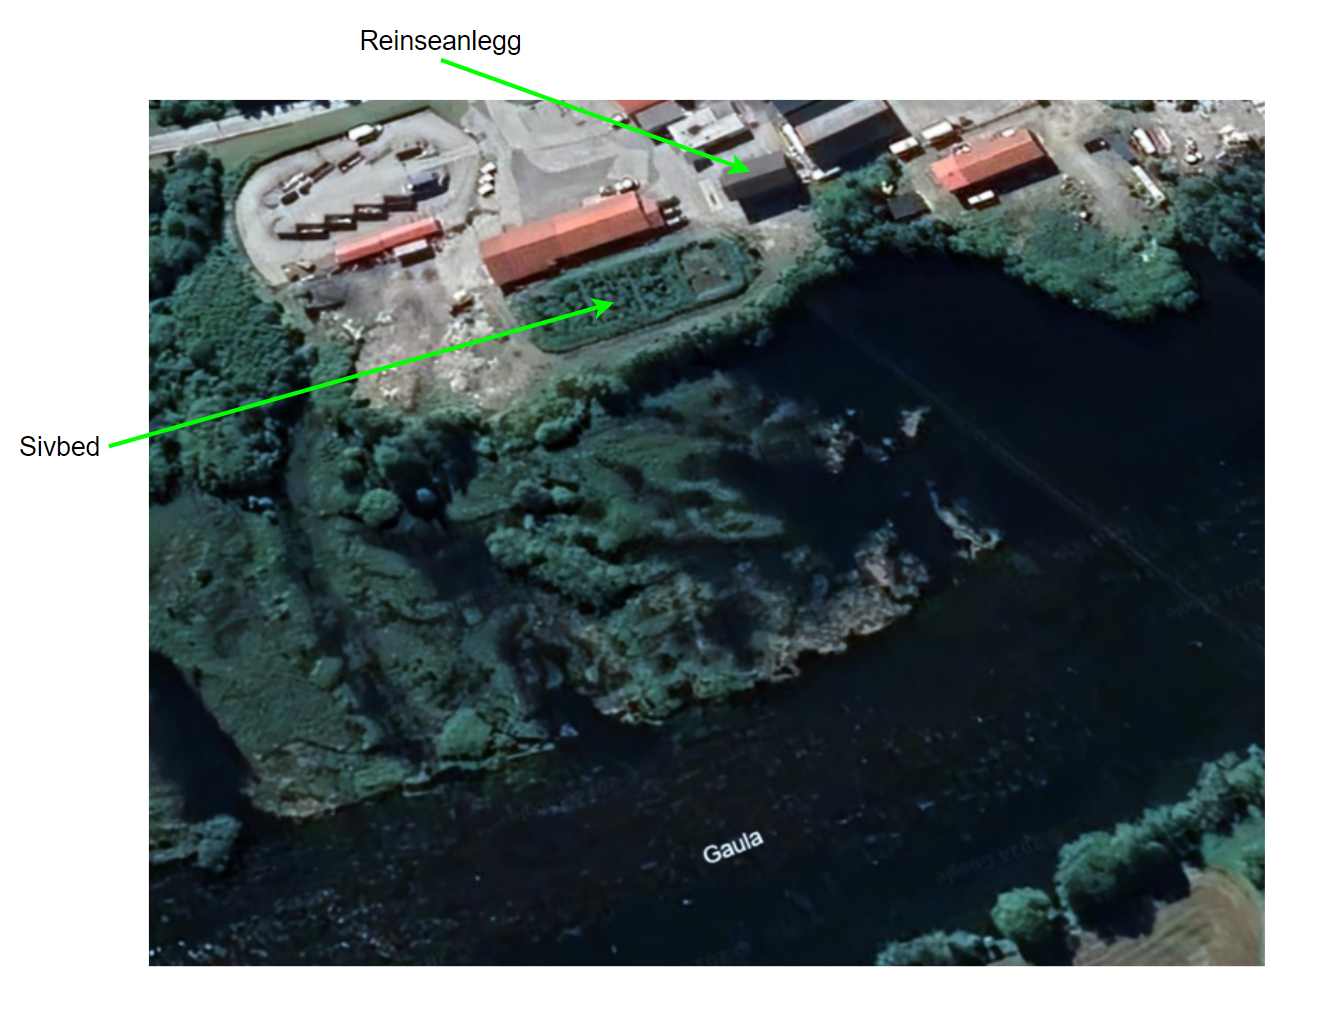
\includegraphics[width=1\textwidth]{Bilder/SatelittFoto.png}
    \caption{Satelittfoto frå Google Earth \citep{Google} }\label{fig:Sivbed}
\end{figure}

\newpage

Vatn frå desse forskjellege dreneringslaga renn vidare til eit pumpehus/kumme.
Pumpehuset er lokalisert tjue meter frå sjølve reinseanlegget og er utstyrt med to pumper og nokre nivåvipper.
Pumpehuset er delt i to og skiljer vatn som kjem frå dei forskjellige dreneringslaga.\newline
I sivbedet er vatn frå djupaste dreneringssone klassifisert som reinsa vatn (sivbed ``reject'') og blir sendt ut til resipient.
Den øvre dreneringssona er forsatt klassifisert som skittent og blir returnert til mottakstanken. \newline \newline \newline \newline \newline

\begin{figure}[htbp]
    \centering
    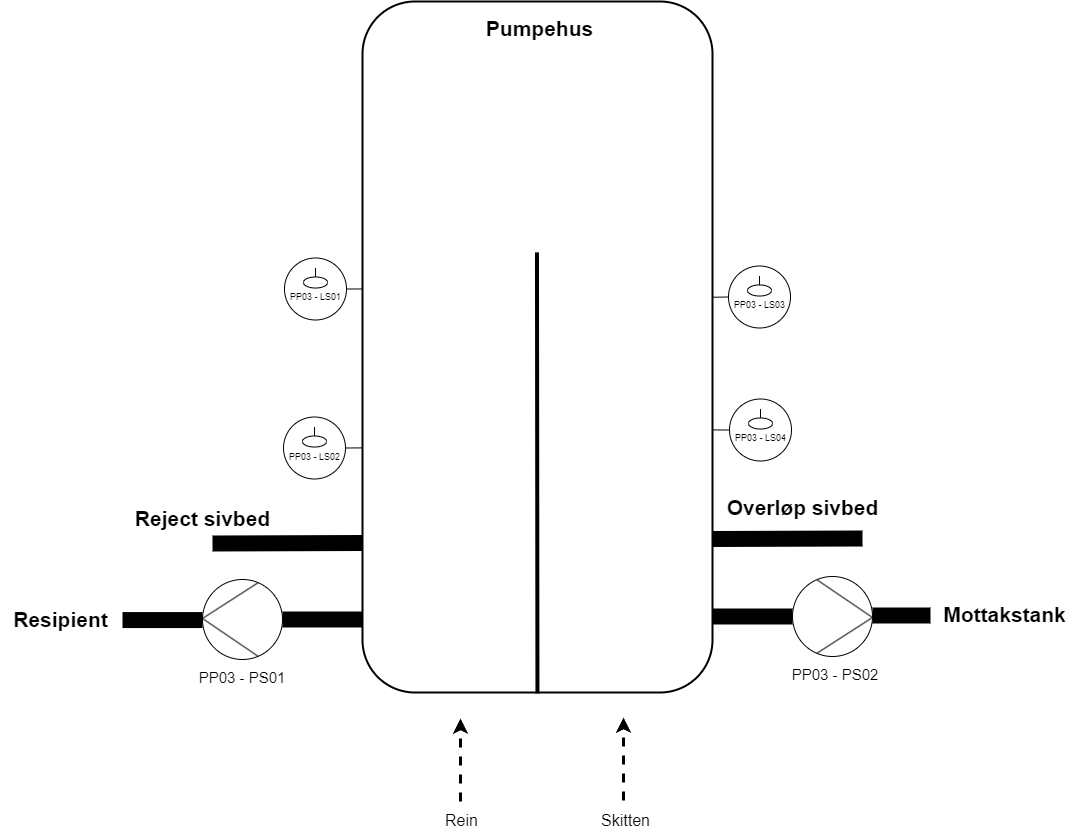
\includegraphics[width=1\textwidth]{Figurar/Pumpehus.drawio.png}
    \caption{\gls{PID} pumpehus}\label{fig:Pumpehus}
\end{figure}

\begin{figure}[htbp]
    \centering
    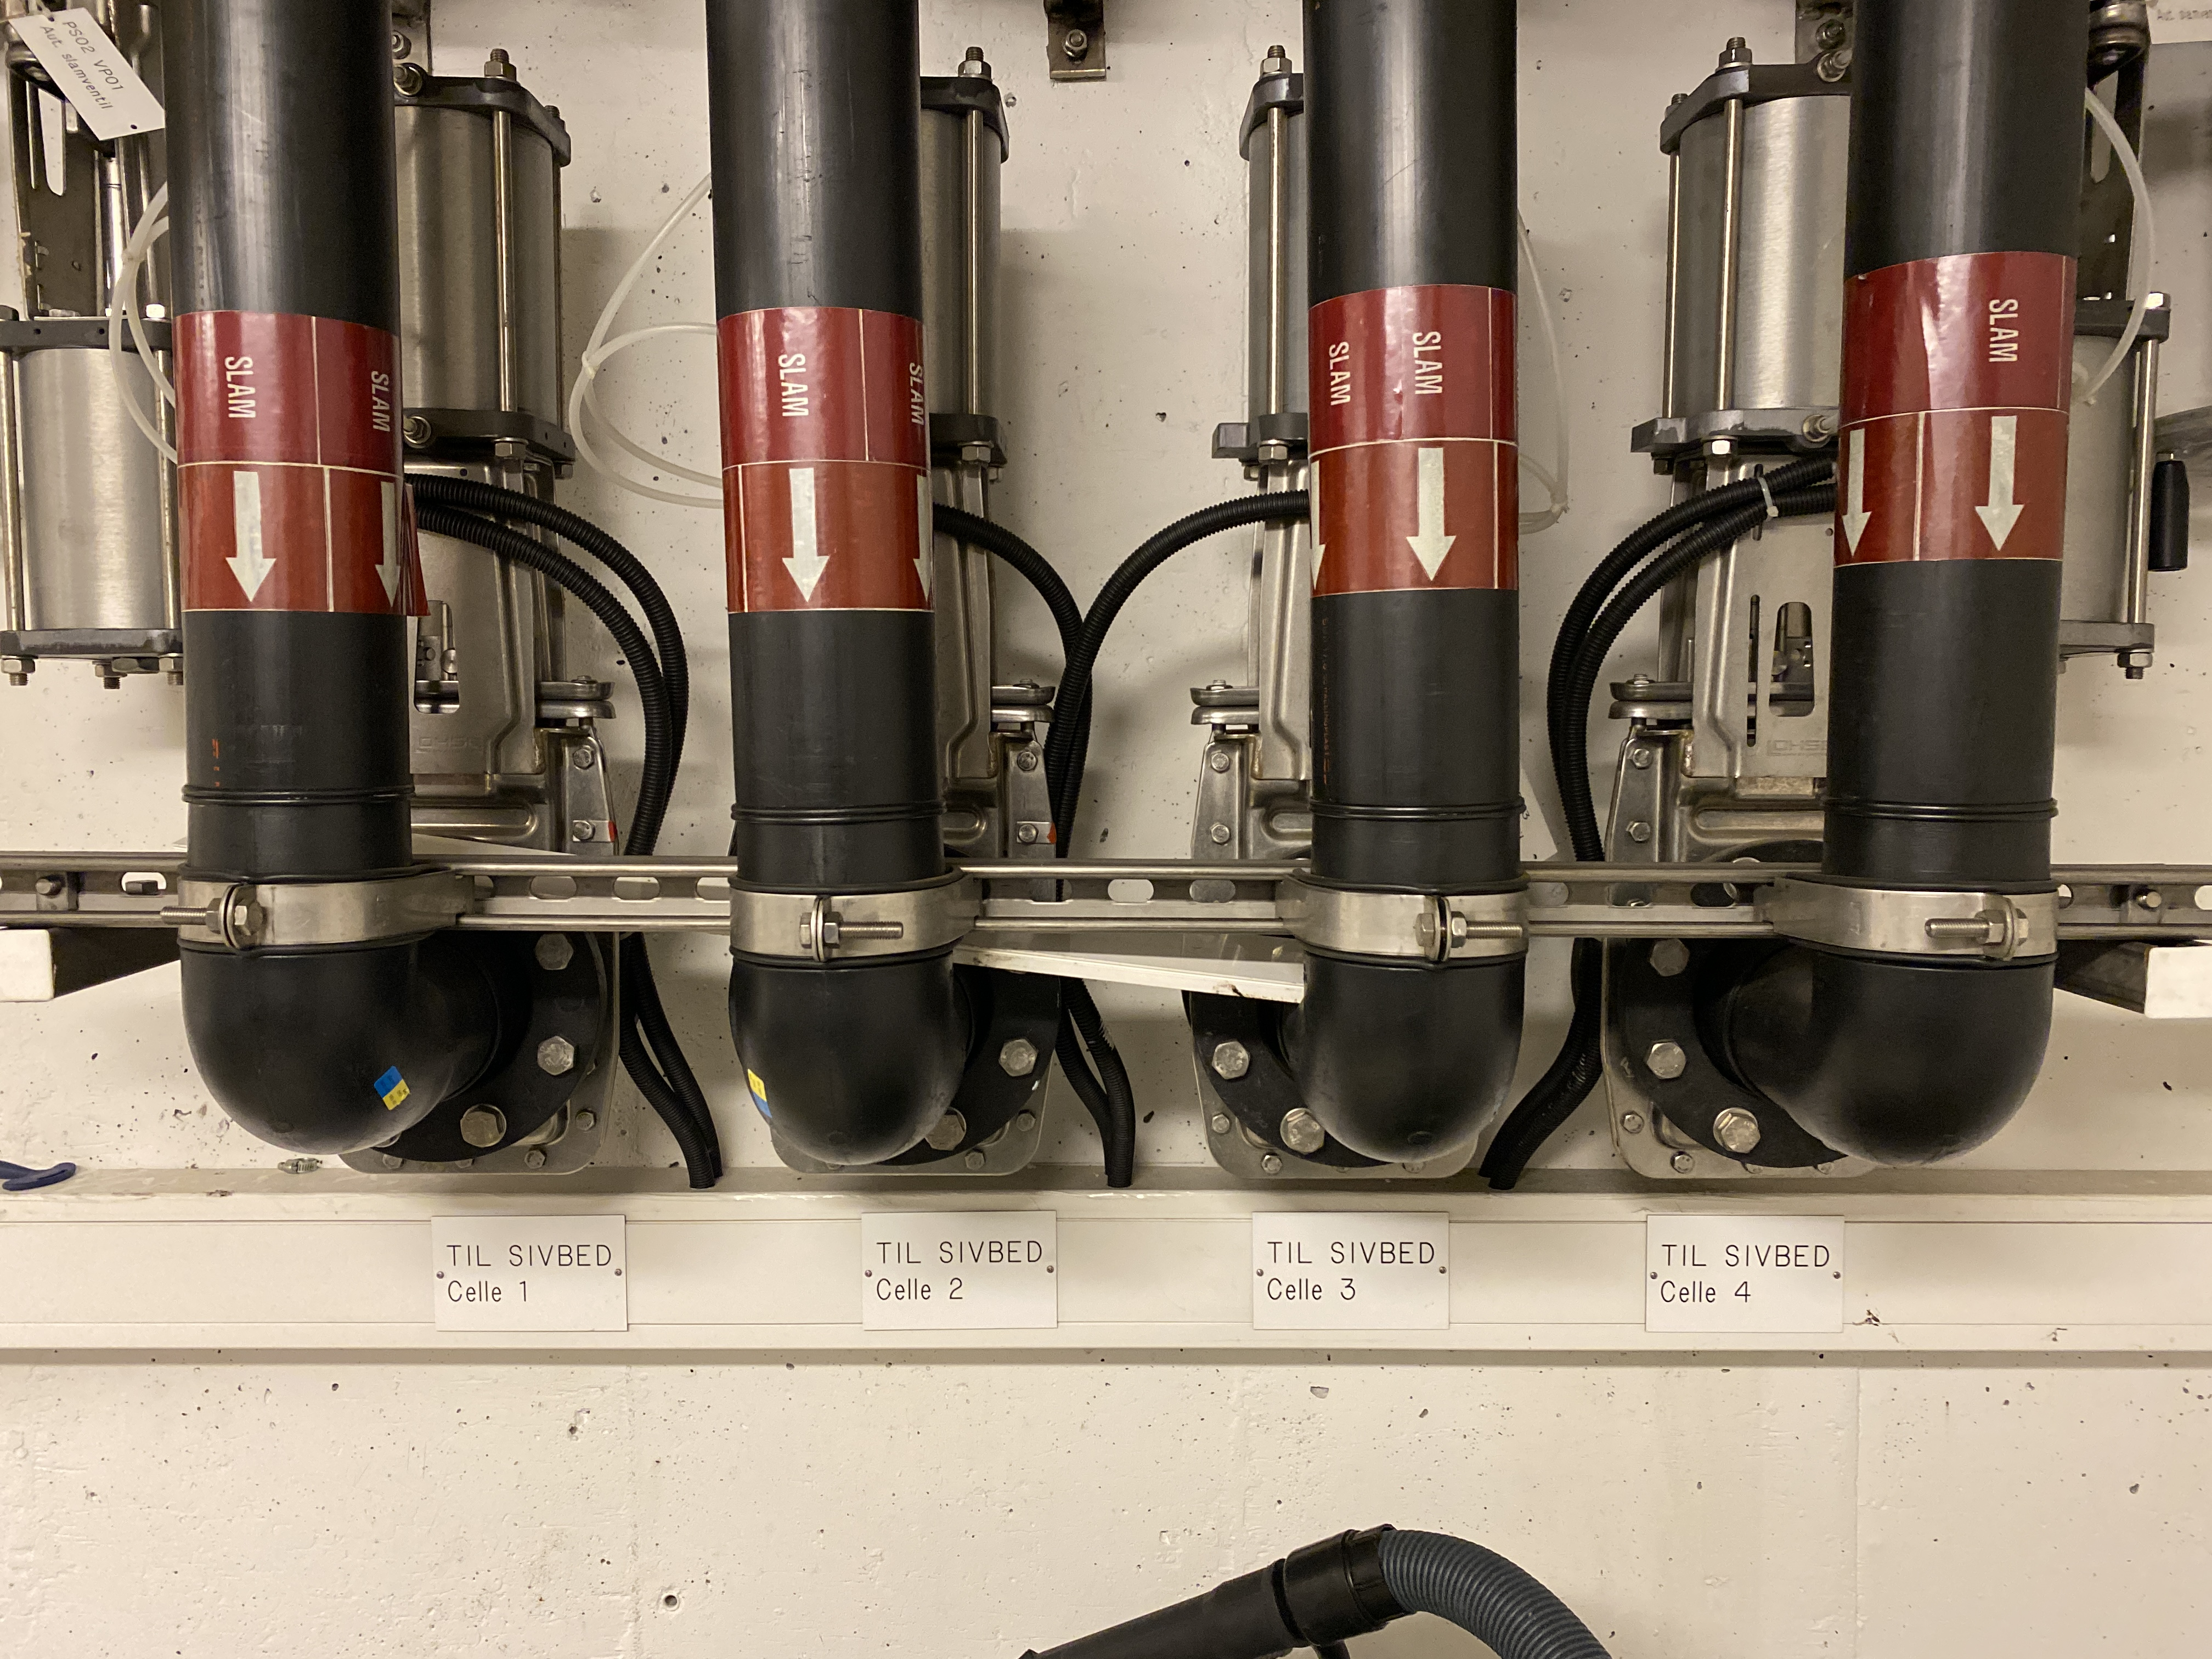
\includegraphics[width=1\textwidth]{Bilder/SivbedSande.jpg}
    \caption{Sivbedventilar}\label{fig:SivbedVentilar}
\end{figure}

\newpage



